%-----------------------------------------------------------------------------------
%	PACKAGES AND OTHER DOCUMENT CONFIGURATIONS
%----------------------------------------------------------------------------------



\documentclass[11pt]{article}

\usepackage[left=2.54cm, right= 2.54cm, top=2.54cm]{geometry}

\usepackage{graphicx}
\usepackage{float}

\setlength{\parindent}{0in}

\newcommand{\Var}{\mathrm{Var}}

\newcommand{\Cov}{\mathrm{Cov}}

\newcommand{\plim}{\rightarrow_{p}}

\usepackage{amsmath, amsfonts}

\usepackage{bm}

% Expectation symbol
\newcommand{\E}{\mathrm{E}}


%----------------------------------------------------------------------------------
%	TITLE AND AUTHOR(S)
%----------------------------------------------------------------------------------

\title{Econ 683 Assignment 1} % The article title


\author{Nathan Mather} % The article author(s) 

\date{\today} % An optional date to appear under the author(s)


%----------------------------------------------------------------------------------
\begin{document}
	
%------------------------------------------------------------------------------
%	TABLE OF CONTENTS & LISTS OF FIGURES AND TABLES
%------------------------------------------------------------------------------
\maketitle % Print the title/author/date block

\setcounter{tocdepth}{2} % Set the depth of the table of contents to show sections and subsections only

%--------------------------------
%      question 1
%--------------------------------

\section{Compreshensin}

\subsection{}

The 1500g threshold is the threshold for diagnosis with “very low birthweight” (VLBW). Below this threshold we would expect babies to receive additional treatment for their diagnosed VLBW. 

\subsection{}

The authors assume that the health of babies just above and just below the 1500g cutoff are not significantly different. Diagnosing based on a cutoff is considered “convention rather than a biologic criteria” which seems to support their assumption.  Additionally, they need to assume that the mother/doctor cannot affect this outcome with birth timing. In other words, they assume a babies position just above to just below 1500g is “as good as random”. 

\subsection{}

The assumption has less support. Babies at 1499g and 1501g will likely have similar outcomes on average. However, as the difference increases, for example, to 1000g and 2000g it is less clear that these babies are not significantly different. 

\subsection{}
Birthweight and VLBW status
\subsection{}
Mortality??????

\subsection{}
National Center for Health Statistics (NCHS) birth cohort linked infant death files 

\subsection{}
They link them by birth information for hospitalized births

\section{Understanding the Model}

\subsection{}
 A dummy variable is an indicator variable that takes the value of one if a given condition is met and      the value of zero if that condition is not met. 
 
 \subsection{}
 VLBW is an indicator for birth weight below 1500g. \\
 so $VLBW_i = 1 $ if $g_i < 1500$ \\
 and  $VLBW_i = 0 $ if $g_i \geq 1500$
 
 \subsection{}
 
  \renewcommand{\theenumi}{\roman{enumi}}
  \begin{enumerate}
  	\item $\E[Y|g=1450] = \alpha_0 + \alpha_1 - \alpha_2 \times 50 $
  	\item $\E[Y|g=1550] = \alpha_0 + \alpha_3 \times 50 $
  	\item$\E[Y|g=1450] = \alpha_0 + \alpha_1 - \alpha_2$
  		\item $\E[Y|g=1501] = \alpha_0 + \alpha_3$
  \end{enumerate}

\subsection{}
The interpretation for $\alpha_2$ is that for babies under 1500g (with $VLBW = 1$) an increase in 1g of birth-weight is associated with an $\alpha_2$ change in $Y_i$, Mortality. 
\\
\\
The interpretation for $\alpha_3$ is that for babies above 1500g (with $VLBW = 0$) an increase in 1g of birth-weight is associated with an $\alpha_3$ change in $Y_i$, Mortality.

\subsection{}

They differ because $\alpha_2$ applies to babies with a VLBW diagnosis and $\alpha_3$ applies to those without. We expect that babies with the VLBW Diagnosis will receive different levels and types of care. 

\subsection{}

The slope below the cutoff, $\alpha_2$ will be less steep than the slope after the cutoff. 
see the graph below. \\
\\ \\ \\ \\ \\ \\ \\ \\ \\ \\ \\ \\ \\ \\ \\ \\ \\ \\ \\ \\ \\ \\ 

\subsection{}
  \renewcommand{\theenumi}{\roman{enumi}}
\begin{enumerate}
	\item The intercept for just below the cutoff, when $VLBW_i = 1$ and $g_i = 1500$, is $\alpha_0 + \alpha_1$. The intercept for just above the cutoff, when $VLBW_i = 0$ and $g_i = 1500$, is $\alpha_0$. 
	 
	 \item The difference between the two, $\alpha_1$, is the effect of having the VLBW diagnosis for a baby on the margin of the 1500 gram cutoff. 
	 
	 \item The difference exists because the formal diagnosis of VLBW leads to different treatments for babies even if their actual weight is roughly the same. For example, more medical procedures or being transfered to a NICU because of the diagnosis would lead to a discrete drop in mortality at 1500g for babies as they move from above to below the 1500g cutoff. 
\end{enumerate}

\subsection{}
$\alpha_0 + \alpha_1-1500\alpha_2$

\subsection{}
This represents the expected mortality or costs for a baby with VLBW  and weighing 0g. This makes no sense because a baby can't weight 0g. I also expect that the linearity assumption starts to break down for babies at the extreme as the survival rate moves to zero. 

\subsection{} 
see the graph below 
\newpage\subsection{}

  \renewcommand{\theenumi}{\roman{enumi}}
\begin{enumerate}
	\item positive 
	\item negative 
	\item negative 
	\item negative 
\end{enumerate}

\section{Running the Regression}
\subsection{}
\begin{enumerate}
	\item $\alpha_0 = .0630851$
	\item $\alpha_1 = -.0095432 $
	\item $\alpha_2 = -.0001364 $
	\item  $\alpha_3 = -.0002238  $
\end{enumerate}

\subsection{}
They are all significant 

\subsection{}
it will change by $-\alpha_1$ so it increases by 0.0095432

\subsection{}
the cost will be $  \frac{4553}{-\alpha_1} =\frac{4553}{0.0095432} = 477,094$  dollars

\subsection{}
The cost I found above is significantly less than \$2.7 million. Additionally the high end of the 95\% confidence interval would put the cost at $ \frac{4553}{0.0052925} = \$ 860,234$. So yes, the additional expenditure seems "worth it". 

\subsection{}

\begin{figure}[H]
	\caption{Gestational Age VS. Birth Wright}\label{fig1}
	\begin{center}
		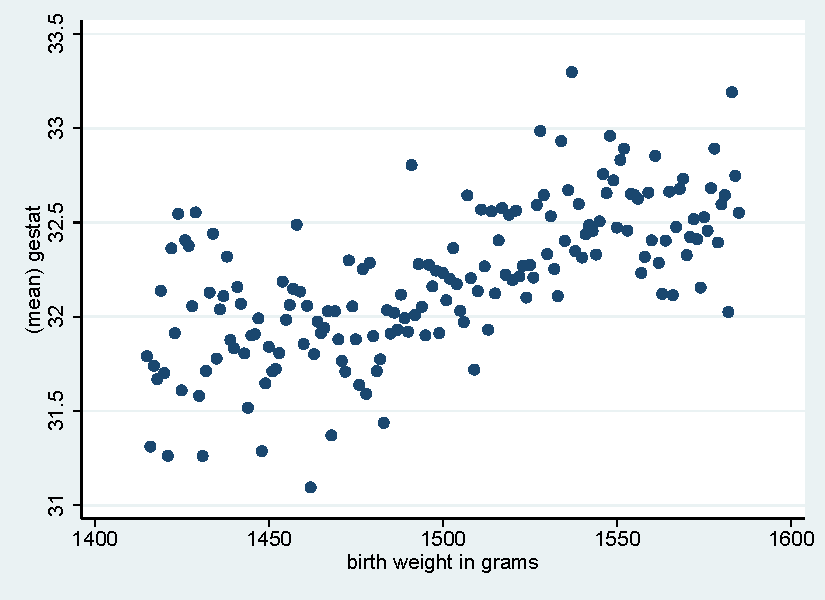
\includegraphics[height=5in,angle=0]{my_ps1_graph.pdf}
	\end{center}
\end{figure}

\begin{enumerate}
	\item Gestational age is increasing with birth-weight
	\item There does not appear to be any significant jump 
	\item if there was a jump in gestational age at 1500g than it would call into question the randomness or exogeneity of the 1500g cutoff????????????????????
\end{enumerate}

\section{Concluding Questions}
\subsection{}
What is novel is the set up for regression discontinuity. The authors have a continuous ovsevable variable of birthweight in grams. They also have a practice of diagnosing VLBW with the fairly hard cutoff of 1500g. The fact that this cutoff is convention rather than biological is on major factor. Another important factor is that this diagnosis actually impacts the level of care these babies receive. Additionally, mothers and doctors are not able to affect birth-weight via birth timing with enough precision to change their VLBW status for babies clost to the cutoff. All of this combines to give a natural experiment setting where babies that are close to the 1500g cutoff can be thought of as being "essentially randomly" assigned to one of the two groups. Babies in the VLBW group receive more treatment and babies out of it receive less.

\subsection{}

\subsection{}
It tells us that the cost of neonatal is probably worth the benefit even if we are only considering the gains in terms of fewer deaths. It also suggests that doctors should review the 1500g cutoff for VLBW or at least procedures for VLBW babies as it seems babies just above the margin could benefit from the care being recieved by babies just below the cutoff. 




%------------------------------------------------
% end doc
%------------------------------------------------
\end{document}
